\documentclass[10pt,a4paper]{article}
\usepackage[margin=22mm]{geometry}
\usepackage[T1]{fontenc}
\usepackage{lmodern,microtype,amsmath,amssymb,booktabs,graphicx}
\usepackage[colorlinks=true,allcolors=blue]{hyperref}
\usepackage{caption}
\captionsetup{font=small,labelfont=bf}
\setlength{\parindent}{0pt}
\setlength{\parskip}{5pt}
\newcommand{\OracleReduction}{41.19}
\newcommand{\WrongIncrease}{8.25}
\newcommand{\KKTError}{1.421\times10^{-14}}
\newcommand{\Idempotence}{4.441\times10^{-16}}
\newcommand{\BeforeBalance}{11.8785}
\newcommand{\AfterBalance}{1.776\times10^{-14}}
\newcommand{\MaxMCZ}{1.014}
\newcommand{\BiasPenalty}{112}
\newcommand{\BiasedRisk}{187.6632}
\newcommand{\FixedRows}{Base & 128.6500 & 1.000000 & 128.7995 & 0.304 \\
Bottom up & 82.2000 & 0.638943 & 81.8688 & -0.859 \\
OLS & 104.7000 & 0.813836 & 104.7081 & 0.017 \\
Oracle & 75.6632 & 0.588132 & 75.2828 & -1.014 \\
Wrong weights & 139.2623 & 1.082489 & 139.4650 & 0.329 \\}
\newcommand{\CalibrationRows}{10 & Sample & 0.9429 & 0.0386 & 0.6981--1.2816 & 25.00\% \\
10 & Half shrinkage & 0.6661 & 0.0040 & 0.6300--0.7167 & 0.00\% \\
10 & Diagonal & 0.6783 & 0.0022 & 0.6609--0.6976 & 0.00\% \\
20 & Sample & 0.6848 & 0.0083 & 0.6172--0.7634 & 1.25\% \\
20 & Half shrinkage & 0.6427 & 0.0017 & 0.6244--0.6661 & 0.00\% \\
20 & Diagonal & 0.6724 & 0.0011 & 0.6610--0.6854 & 0.00\% \\
50 & Sample & 0.6263 & 0.0027 & 0.6021--0.6551 & 0.00\% \\
50 & Half shrinkage & 0.6365 & 0.0010 & 0.6250--0.6496 & 0.00\% \\
50 & Diagonal & 0.6695 & 0.0007 & 0.6616--0.6760 & 0.00\% \\
200 & Sample & 0.5968 & 0.0006 & 0.5906--0.6051 & 0.00\% \\
200 & Half shrinkage & 0.6305 & 0.0005 & 0.6259--0.6368 & 0.00\% \\
200 & Diagonal & 0.6673 & 0.0003 & 0.6635--0.6711 & 0.00\% \\}

\title{LoadCoherent: aggregation consistency and covariance uncertainty\\
in synthetic district heat-load predictions}
\author{}
\date{Reproducible computational study, 8 October 2026}
\begin{document}
\maketitle
\vspace{-2em}
\begin{abstract}
Aggregation constraints provide a useful check on district heat-load predictions,
but satisfying them does not establish predictive accuracy. This study implements
covariance-weighted reconciliation using Cholesky whitening and QR factorization.
A synthetic four-building network permits analytical evaluation of prediction
risk and independent verification by a constrained linear solve. Oracle weights
reduce the sum of node mean-square errors by \OracleReduction\%, whereas a
deliberately misspecified weight increases it by \WrongIncrease\% despite
coherence. Independent finite-calibration experiments show a tradeoff: fixed
diagonal shrinkage limits small-sample variance, but retains estimation bias as
sample size grows. The study separates numerical projection error, statistical
estimation error and untested physical validity. It evaluates an established
method rather than proposing a new forecasting algorithm.
\end{abstract}

\section{Question and thermal assumptions}
The research question is: when is an aggregation-consistent heat-load prediction
less accurate than its unconstrained input? This is relevant when building,
district and plant forecasts are generated separately. Topic selection arose
from DTU Advanced Time Series Analysis lecture material on hierarchical
reconciliation and heat-load forecasting. All network parameters, experiments,
code and illustrations here are original synthetic constructions; no private
course material or measured load data is reproduced.

Four buildings are partitioned into north (1,2) and south (3,4). Building demand
is the quasi-steady heat loss
\begin{equation}
 b_i(t)=U_i[T_{\rm in}-T_{\rm out}(t)],\quad
 T_{\rm out}(t)=4+5\sin(2\pi t/24),\quad T_{\rm in}=21.
 \label{eq:thermal}
\end{equation}
Temperatures are in degrees Celsius, $t$ in hours, and
$U=(1.2,0.8,1.5,1.0)$ in kW/K. Perfect demand tracking, negligible storage and
lossless pipes are assumed. With node order plant, north, south, 1,2,3,4,
\begin{equation}
 y=S b,\qquad S=\begin{bmatrix}S_{\rm top}\\I_4\end{bmatrix}
 \in\mathbb R^{7\times4},\qquad
 S_{\rm top}=\begin{bmatrix}1&1&1&1\\1&1&0&0\\0&0&1&1\end{bmatrix}.
 \label{eq:summing}
\end{equation}
The last four rows are the identity. Equation~\eqref{eq:thermal} is an algebraic
thermal model: it neither resolves transient conduction nor provides a district
heating design calculation. Its role is to supply a coherent, positive reference
signal for evaluating a statistical projection.

\section{Reconciliation and analytical risk}
Let $\hat y=y+e$, with $\mathbb E e=\mu$ and $\operatorname{Cov}(e)=V$.
For any symmetric positive-definite weight $W$, define
\begin{equation}
 \tilde y=S\arg\min_z(Sz-\hat y)^TW^{-1}(Sz-\hat y)=P_W\hat y.
 \label{eq:projection}
\end{equation}
This is the weighted reconciliation framework of
Wickramasuriya et al.~\cite{mint}; a public exposition is given by
Hyndman and Athanasopoulos~\cite{fpp}. For full-column-rank $S$,
$P_WS=S$ and $P_W^2=P_W$. Thus the exact signal is preserved, and errors transform
as $P_We$. Taking the second moment gives the per-node risk used here:
\begin{equation}
 r_j=[P_WVP_W^T]_{jj}+[P_W\mu]_j^2,\qquad R=\sum_{j=1}^{7}r_j.
 \label{eq:risk}
\end{equation}
\newpage

\section{Implementation and reproducible experiments}
\subsection{Algorithm and verification}
For $W=LL^T$, form $A=L^{-1}S=QR$ by Cholesky whitening and reduced QR.
Solve $RG=Q^TL^{-1}$ with triangular solves and set $P_W=SG$.
Application uses $S(G\hat y)$, or its transposed batch equivalent.
No explicit inverse or normal-equation matrix is constructed. The dense Python
implementation uses NumPy and SciPy. Factoring weights costs $O(n^3)$; this
implementation targets small hierarchies, and no speed advantage is claimed.
It rejects nonfinite or complex data, incompatible shapes, relative weight
eigenvalues at or below $10^{-12}$, and relative whitened singular values at or
below $10^{-12}$. These cutoffs are safeguards rather than accuracy certificates.

An independent saddle-point computation solves
\begin{equation}
 \begin{bmatrix}V&S\\S^T&0\end{bmatrix}
 \begin{bmatrix}\lambda\\z\end{bmatrix}
 =\begin{bmatrix}\hat y\\0\end{bmatrix},\qquad \tilde y=Sz,
 \label{eq:kkt}
\end{equation}
for the oracle case. Tests additionally cover a scalar inverse-variance example,
weighted orthogonality, scale invariance, batch application, projection
identities, covariance estimation, invalid inputs and coherent bias.
The installed-wheel tests and complete numerical-output reproduction run on
Windows and Ubuntu in CI. The manuscript build reads numerical tables directly
from the results JSON, records input/PDF hashes and enforces a five-page limit.

\subsection{Specified error population}
Independent Gaussian error vectors use $V=FF^T+\operatorname{diag}(d^2)$, where
\begin{equation}
 F=\begin{bmatrix}
 7&0&0\\2&4&0\\3&0&3\\1&2&0\\1.5&-1&0\\1&0&1.5\\2&0&-1
 \end{bmatrix},\qquad
 d=\begin{bmatrix}3&2&2.5&1&1.2&1.1&1.5\end{bmatrix}^T.
 \label{eq:population}
\end{equation}
Factor coefficients and $d$ are in kW. Shared factors represent correlated
forecast errors, not simulated random heat sources. They are deliberately not
coherent across aggregation levels. The positive diagonal term ensures $V$ is
positive definite. No forecasting model is trained: the experiment supplies its
prediction errors directly, isolating reconciliation from model selection.

Five fixed references are evaluated: unreconciled base; bottom up using only
the last four forecasts; OLS ($W=I$); oracle ($W=V$); and wrong weights
$W=\operatorname{diag}(0.01,1,1,100,100,100,100)$.
The last choice over-trusts the plant and is a deliberate stress test.
For $\mu=0$, equation~\eqref{eq:risk} gives the exact population risk.
The sum includes overlapping aggregate targets; it is a forecasting loss,
not a conserved thermal quantity. Node-level results are also recorded.

\subsection{Calibration and sampling protocol}
NumPy seed 20261008 spawns separate test, calibration and display generators.
For each sample size $N\in\{10,20,50,200\}$, 80 independent calibration sets
are drawn. The same set serves three estimators for a paired comparison:
\begin{equation}
 \hat V=\frac{1}{N-1}\sum_{k=1}^{N}(e_k-\bar e)(e_k-\bar e)^T,\qquad
 W_\alpha=(1-\alpha)\hat V+\alpha\operatorname{diag}(\hat V),
 \label{eq:shrinkage}
\end{equation}
with $\alpha=0,1/2,1$. Half-shrinkage is fixed in advance, not estimated to
minimize reported test risk. Each fitted $P_W$ is evaluated analytically against
the known $V$, so conditional risks have no test-sample Monte Carlo noise.
Separately, 60,000 test errors validate the five fixed-method risks. For these
zero-mean Gaussian errors, the analytic standard error of the mean total
squared loss is $[2\operatorname{tr}\{(P_WVP_W^T)^2\}/60000]^{1/2}$.
The illustrative load path uses 48 hourly points and independent error draws;
it is not a temporally correlated forecast simulation.
\newpage

\section{Measured results}
\begin{table}[h!]
\centering\small
\caption{Fixed weights: analytical risk and independent Monte Carlo check.
Risk and sampled MSE have units kW$^2$; $z$ is the discrepancy divided by its
analytic Monte Carlo standard error.}
\begin{tabular}{lrrrr}\toprule
Method & Exact $R$ & $R/R_{\rm base}$ & Sampled MSE & $z$\\\midrule
\FixedRows
\bottomrule\end{tabular}
\label{tab:fixed}
\end{table}
Oracle weights reduce expected all-node error by \OracleReduction\%, but
wrong weights increase it by \WrongIncrease\%. Thus coherence alone does not
imply improvement. The largest absolute Monte Carlo discrepancy is
\MaxMCZ\ standard errors. The QR/KKT forecast difference is
$\KKTError$ kW and the maximum entry of $P^2-P$ is $\Idempotence$.
Across the illustrative path, the maximum absolute aggregation residual
decreases from \BeforeBalance\ kW to $\AfterBalance$ kW.

\begin{figure}[h!]
\centering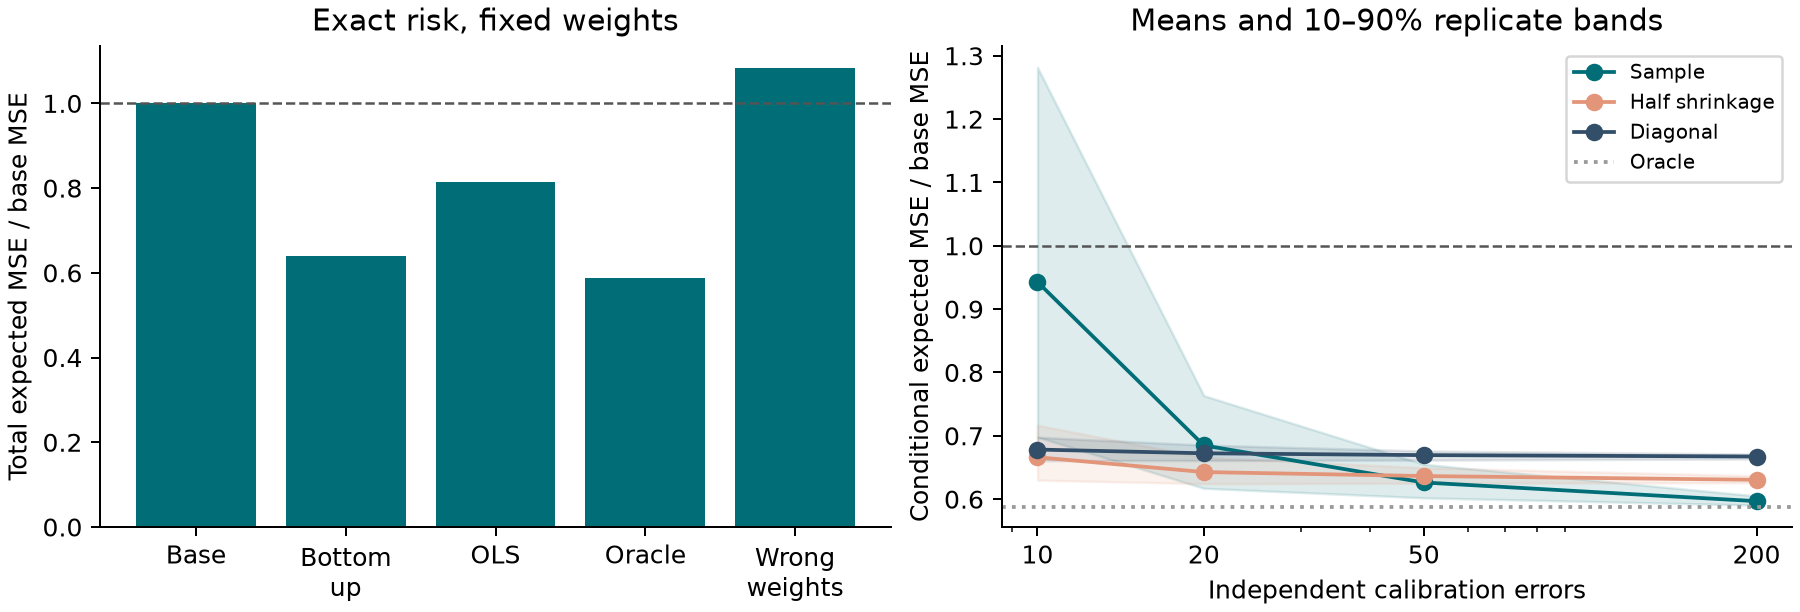
\includegraphics[width=\linewidth]{../examples/results/risk.png}
\caption{Exact risk of fixed methods (left) and calibration sensitivity (right).
Lines show means over 80 calibration sets; shaded areas show their 10th--90th
percentiles, not confidence intervals for the means.}
\label{fig:risk}
\end{figure}

\begin{table}[h!]
\centering\small
\caption{Conditional risk ratio across independent calibration sets. SE is the
standard error of the replicate mean; the final column is the observed fraction
of sets with risk above unreconciled base risk.}
\begin{tabular}{rlrrrr}\toprule
$N$ & Estimator & Mean & SE & 10th--90th percentile & Worse\\\midrule
\CalibrationRows
\bottomrule\end{tabular}
\label{tab:calibration}
\end{table}
At $N=10$, the sample estimator exceeds base risk in 20 of 80 sets. Neither
shrinkage estimator does so in these recorded sets, which does not prove a
universal bound. At $N=200$, the sample estimator has lower mean risk than fixed
half-shrinkage. This reversal reflects covariance estimation variance at small
$N$ and persistent distortion from a fixed diagonal shrinkage target at large
$N$. The study does not optimize the shrinkage fraction or extrapolate beyond
the specified population and sizes.
\newpage

\section{Discussion, limitations and reproducibility}
\begin{figure}[h!]
\centering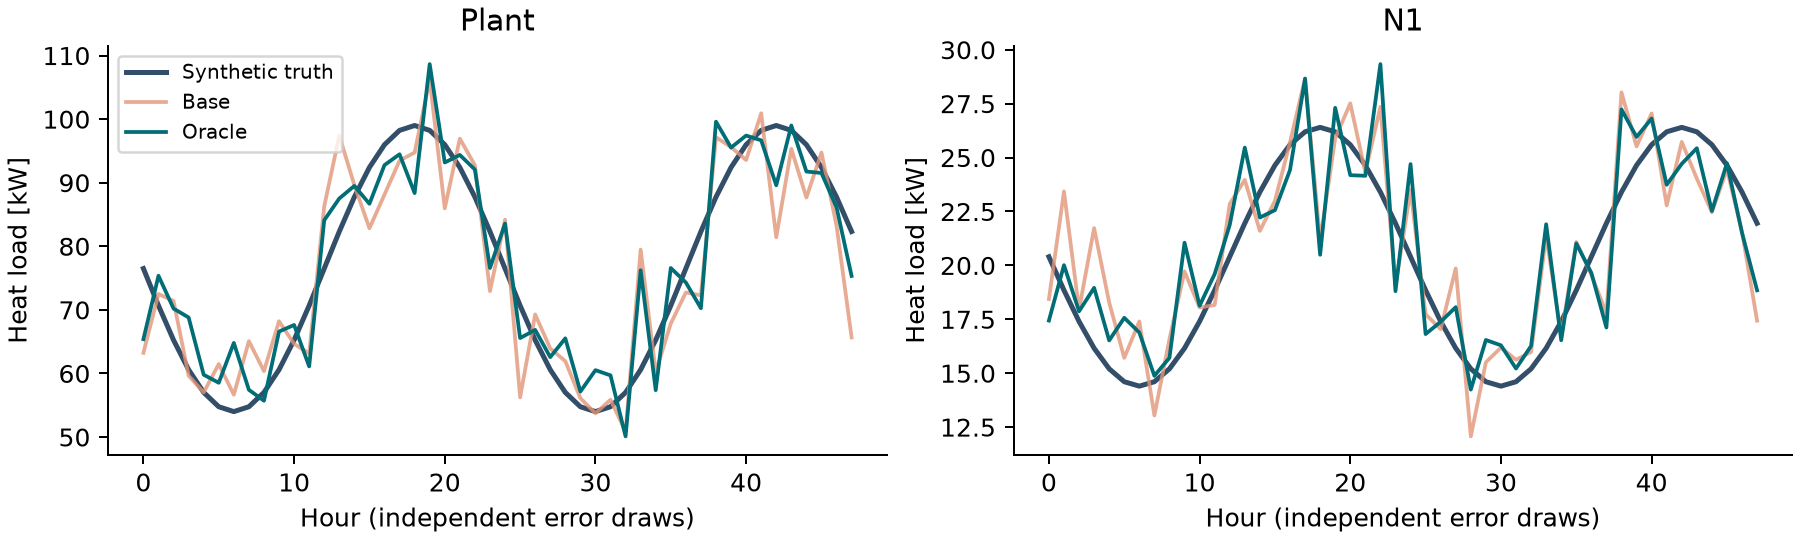
\includegraphics[width=0.94\linewidth]{../examples/results/path.png}
\caption{Illustrative synthetic demand at the plant and one building.
Oracle reconciliation uses known error covariance. This single path visualizes
the construction; the analytical risk study supports accuracy comparisons.}
\label{fig:path}
\end{figure}

\textbf{Bias is a separate problem.} Any coherent bias $\mu=S\delta$ survives:
$P_W\mu=\mu$. Setting every component of $\delta$ to 2 kW gives
$\mu=(8,4,4,2,2,2,2)^T$ kW. The oracle risk then becomes
\BiasedRisk\ kW$^2$, including a \BiasPenalty\ kW$^2$ bias penalty.
Centering calibration errors estimates covariance but does not subtract bias
from subsequent forecasts. Linear reconciliation can also produce negative
loads; a small counterexample is included in the test suite. Nonnegative
constraints would require a different optimization problem.

\textbf{Discrete error and continuum error.} The KKT comparison and projection
identities verify finite-dimensional numerical calculations to roundoff scale.
Finite-calibration risk concerns statistical estimation, not floating-point
error. Equation~\eqref{eq:thermal} is evaluated analytically without spatial or
temporal discretization; there is no continuum mesh-error estimate or PDE
convergence claim. The hourly display is a sampling choice, not a time integrator.

\textbf{Physical validity and scope.} No measurements validate these results.
Pipe storage/losses, uncertain topology, controls, occupancy and time-correlated
errors would change the model. Only one hierarchy and one fixed Gaussian
covariance are studied. The oracle needs unknown population information.
Replicate fractions are finite-experiment outcomes; half-shrinkage is not
asserted to be optimal.

\textbf{Reproduction.} Install and execute from the repository root:
\begin{quote}\small\ttfamily
python -m pip install -e ".[dev]"\\
loadcoherent --output examples/results\\
python scripts/check\_samples.py\\
python -m pytest -q\\
python paper/build.py --engine pdflatex
\end{quote}
CSV files contain calibration risks and paths; JSON contains per-node risks,
matrices and diagnostics. CI checks compilation and page count; hashes bind the
paper to the numerical inputs. Every rendered page must also be inspected.

\section{Conclusion}
Aggregation checks and accuracy checks answer different questions. Weighted QR
enforces the declared constraints, while covariance choice determines risk.
Fixed shrinkage helps the smallest calibration set; sample covariance performs
better at the largest tested size. Neither result validates a real network.

\begin{thebibliography}{9}\small
\bibitem{mint} S. L. Wickramasuriya, G. Athanasopoulos and R. J. Hyndman.
Optimal forecast reconciliation for hierarchical and grouped time series
through trace minimization. \emph{Journal of the American Statistical Association},
114(526):804--819, 2019. \href{https://doi.org/10.1080/01621459.2018.1448825}{doi:10.1080/01621459.2018.1448825}.
\bibitem{fpp} R. J. Hyndman and G. Athanasopoulos.
\emph{Forecasting: Principles and Practice}, 3rd ed., OTexts, 2021.
Section 11.3: \href{https://otexts.com/fpp3/reconciliation.html}{Forecast reconciliation}.
\end{thebibliography}
\end{document}
